\chapter{Results}
The following structure corresponds to project instruction.

% Example: insert image
% \includegraphics{fig/NameOfTheFileWithoutExtension}

\section{Load VTK files and make the basic menu} 

\textbf{Header information from VTK file.}

\begin{table}[h]
	\ttfamily
	\small
	\begin{tabular}{l|l}
		1 & \# vtk DataFile Version 3.0     \\
		2 & vtk output                      \\
		3 & ASCII                           \\
		4 & DATASET STRUCTURED\_POINTS      \\
		& DIMENSIONS 256 256 230          \\
		& SPACING 1 1 1                   \\
		& ORIGIN 0 0 0                    \\
		5 & POINT\_DATA 15073280            \\
		& SCALARS scalars unsigned\_short \\
		& LOOKUP\_TABLE default          
	\end{tabular}
\end{table}

\noindent
\textbf{1} File version and identifier.\\
\textbf{2} Character string header terminated with \textbackslash n (max. 256 characters).\\
\textbf{3} File format: ASCII or BINARY.\\
\textbf{4} Dataset structure describing the geometry and topology of the dataset. Available structures: STRUCTURED\_POINTS, STRUCTURED\_GRID, UNSTRUCTURED\_GRID, POLYDATA, RECTILINEAR\_GRID, FIELD.\\
\textbf{5} Dataset attributes, number of data items = number of points in the dataset; dimension x*y*z = POINT\_DATA

The data in the given files is compressed by means of storing a single grayscale value for each point. Apart from this, no futher compression to file is applied.

\section{Planes for different views}

\begin{figure}
	\centering
	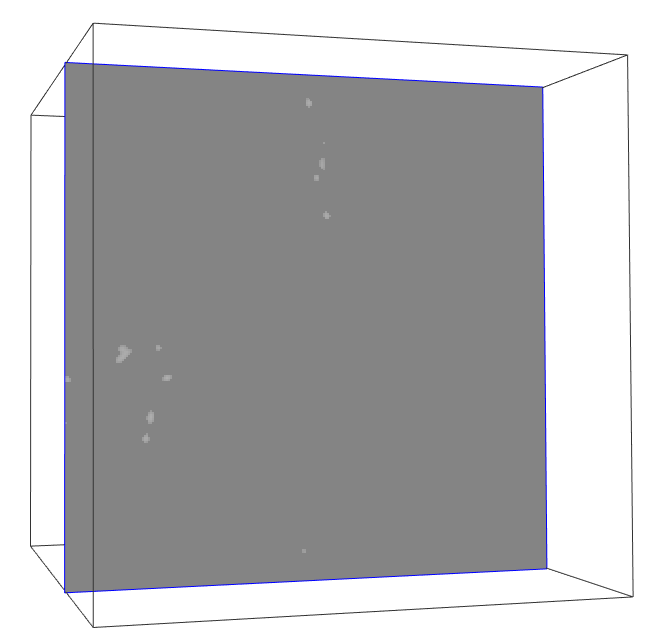
\includegraphics[scale=0.3]{fig/image-plane}
	\caption{Coronal view for segmented image.}
	\label{fig:image-plane}
\end{figure}

A class vtkImagePlaneWidget was used to show the cut from the segmented data (Figure \ref{fig:image-plane}). In segmented image view we can show sagittal, transversal and coronal views by pressing S, T and C keys respectively. The segmented image is then hidden in order to show a cut and scrolling through the slices is possible by pressing + and - keys.

\section{Marching cubes and building the skeleton}

\begin{figure}
	\centering
	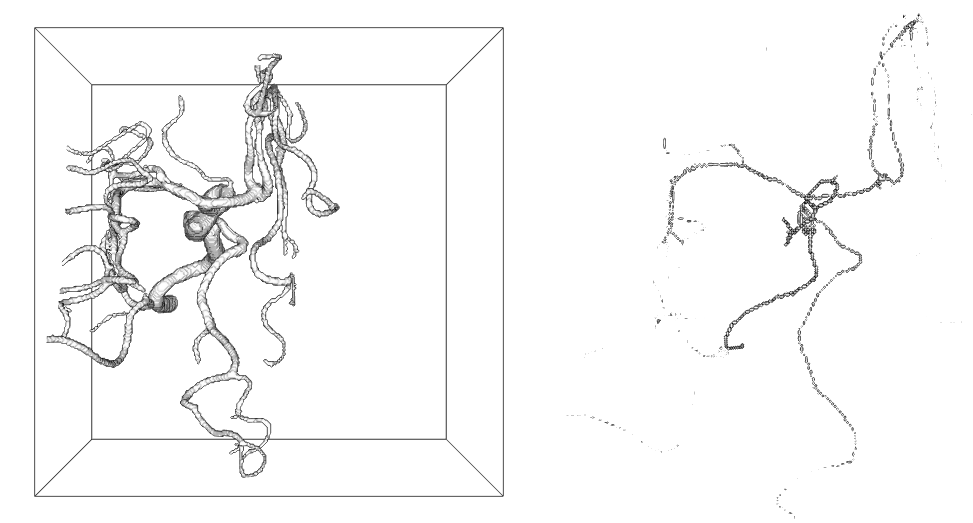
\includegraphics[scale=0.6]{fig/segmented-skeleton}
	\caption{vtkContourFilter used to render segmented and skeleton mesh.}
	\label{fig:segmented-skeleton}
\end{figure}

\begin{figure}
	\centering
	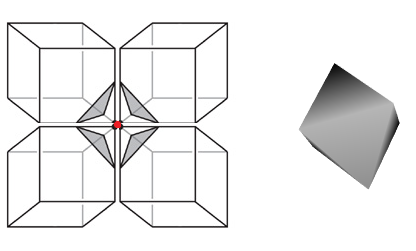
\includegraphics[scale=0.6]{fig/marching-cubes-1-point}
	\caption{Only one voxel with non-zero value (all other voxels are set to 0.)}
	\label{fig:marching-cubes-1-point}
\end{figure}

\begin{figure}
	\centering
	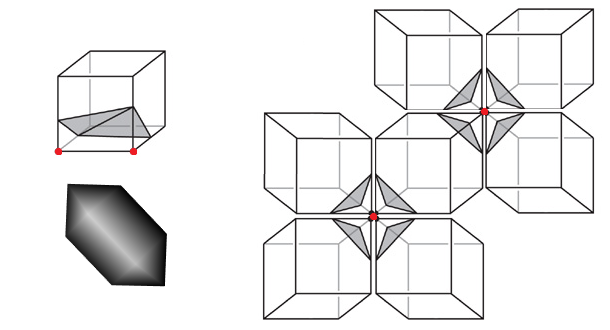
\includegraphics[scale=0.6]{fig/marching-cubes-2-points}
	\caption{Two voxels with non-zero value (all other voxels are set to 0.)}
	\label{fig:marching-cubes-2-points}
\end{figure}

% label doesn't work :/
\begin{lstlisting}[caption={A sample from skeleton file},label={lst:sample-skeleton}]
0 0 0 0 0 0 0 0 0 
0 0 0 0 0 0 14 0 0 
0 0 0 0 0 0 0 0 0 
\end{lstlisting}

A class vtkContourFilter was used to render segmented and skeleton images as they are in provided files (Figure \ref{fig:segmented-skeleton}).
The visualized skeleton path is not continuous due to provided data that was processed by vtkContourFilter. The values occur alone, the adjacent ones have value zero (Listing 1.1). If this situation occurs, there is a small cube mesh built around this voxel (Figure \ref{fig:marching-cubes-1-point}). Similar case is with two voxels with non-zero value (Figure \ref{fig:marching-cubes-2-points}).

TODO : -	Build the skeleton using the vtkTubeFilter (single tube should be used for a single branch. A branch in the skeleton image consists of neighboring voxels that have 2 neighbors (they are part of the path), and start and end voxel (they have either 1 or mode than 2 neighbors in their 3D neighborhood). In order to make a tube, the voxels have to be entered in a SEQUENTIAL order from one (start) voxel to the other (end) voxel).\\
-	How does the skeleton look like? Are the branches smooth? Why?\\
-	Make the branches smooth.\\

\begin{figure}
	\centering
	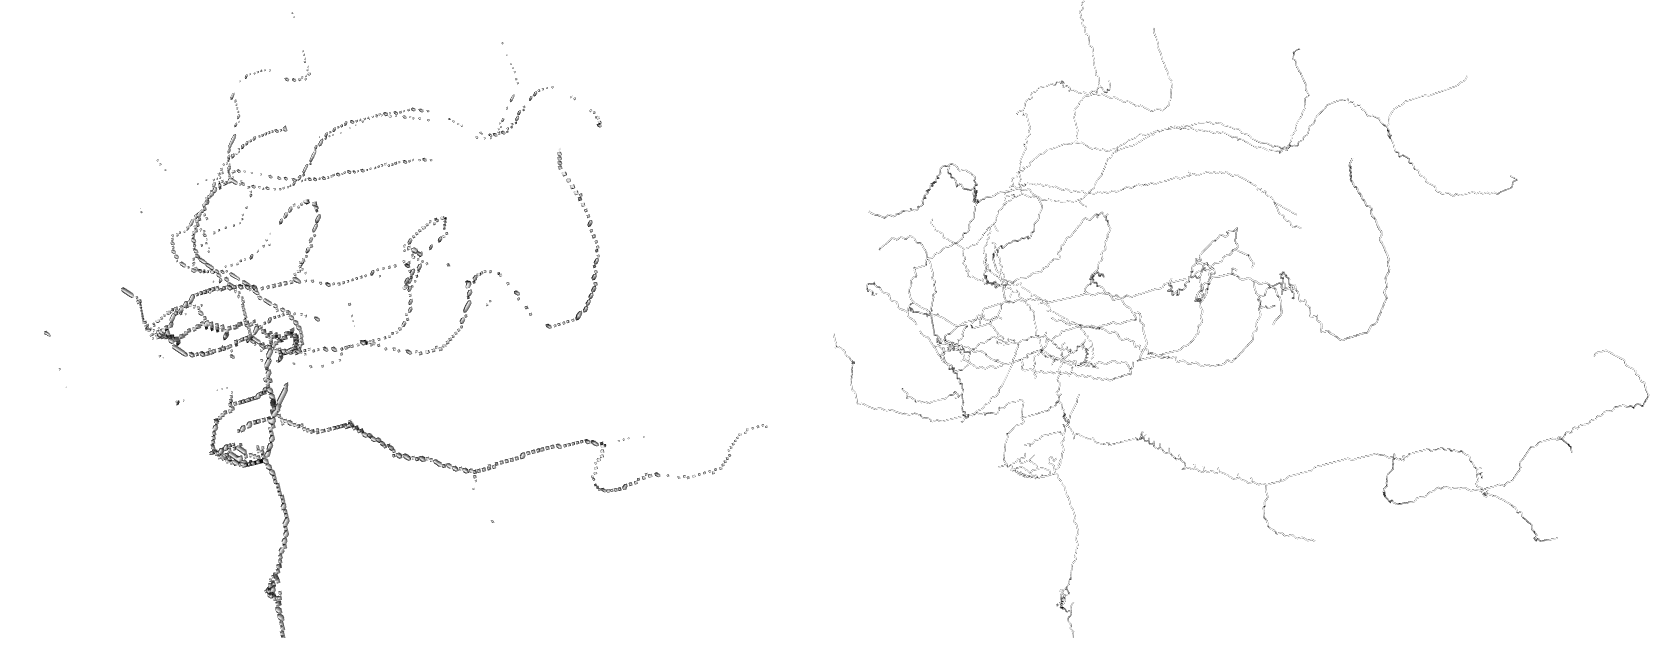
\includegraphics[scale=0.4]{fig/skeleton-basic-tubed}
	\caption{Skeleton basic (left) and tubed (right) view.}
	\label{fig:skeleton-basic-tubed}
\end{figure}

\begin{figure}
	\centering
	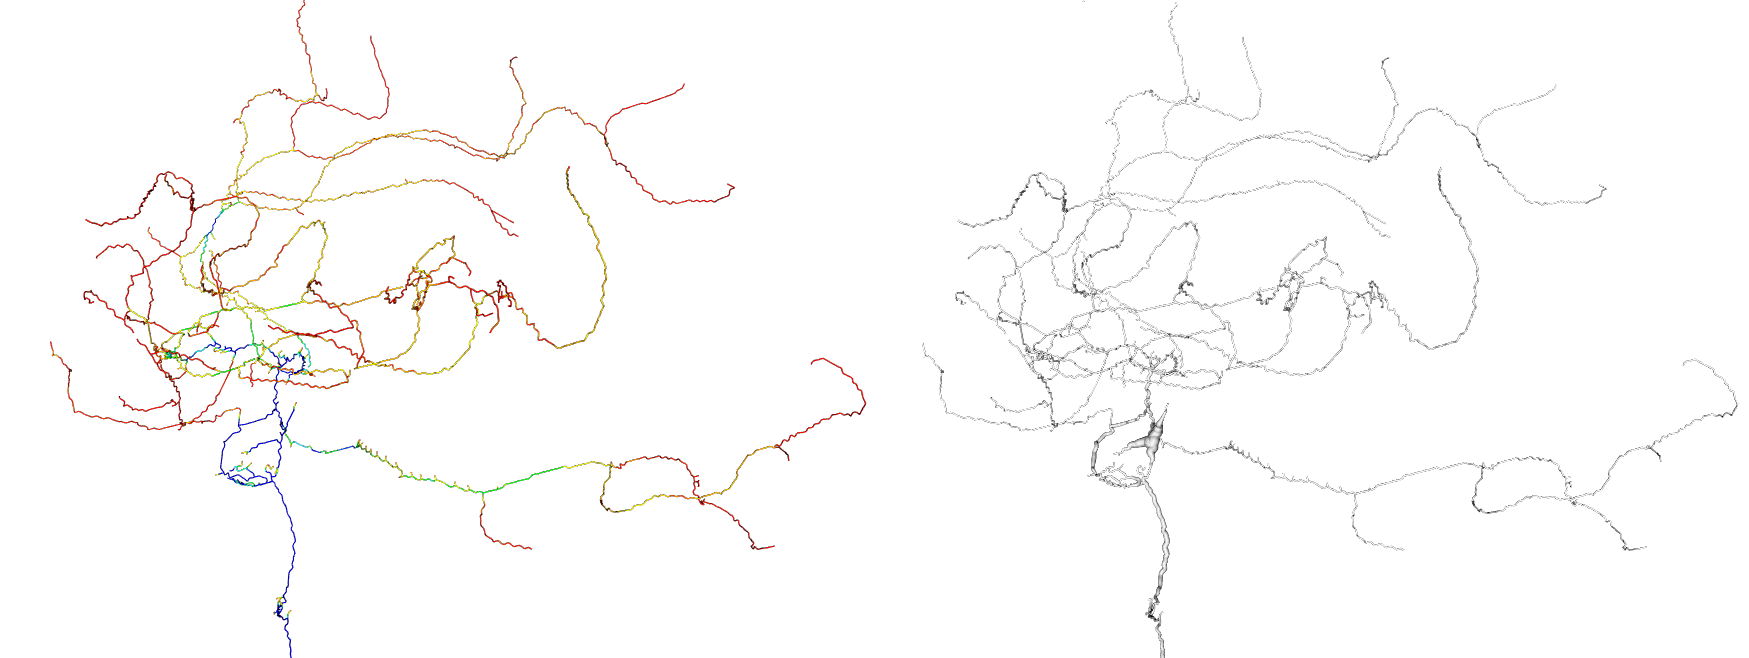
\includegraphics[scale=0.4]{fig/skeleton-colored-radius}
	\caption{Skeleton colored (left) and with varying radius (right) view.}
	\label{fig:skeleton-colored-radius}
\end{figure}

\section{Volume visualization}

\begin{figure}
	\centering
	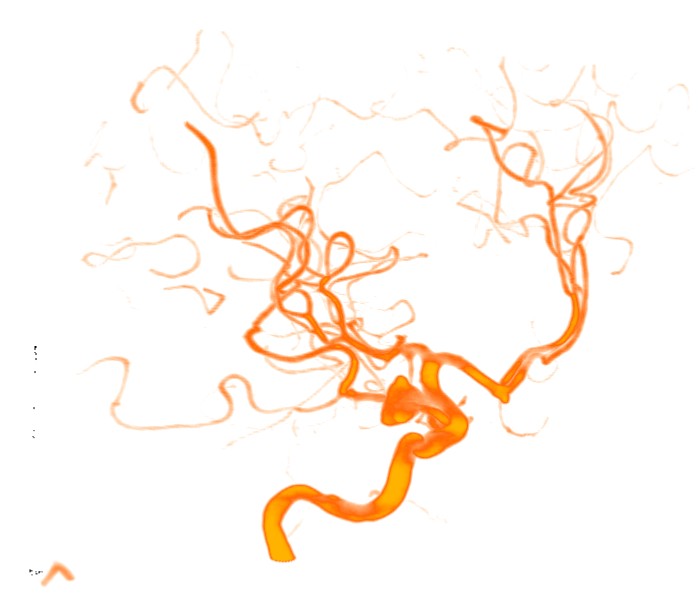
\includegraphics[scale=0.4]{fig/volume-rendering}
	\caption{Volume rendering.}
	\label{fig:volume-rendering}
\end{figure}

The volume visualization was obtained by using vtkVolumeRayCastMapper with vessels\_data.vtk (Figure \ref{fig:volume-rendering}). The crucial part was to set proper RGB points in vtkColorTransferFunction which correspond to luminance values from the VTK file.

Because rendering requires complex computation, the image is blurred while rotating and it regains the focus when rotation stops.

\section{Point picker and distance calculation}

For any skeleton mesh there is a possibility to measure Euclidean distance. An Ecuclidean distance between two voxels can be measured by clicking on skeleton mesh. The result will be displayed in bottom right corner of the window. Reset of selected start voxel can be performed with "x" key.

\section{Visualization}

We distinguish 6 meshes:
\begin{itemize}
	\item Key "1": skeleton basic view, by reading directly from file without modifications except vtkContourFilter (Figure~\ref{fig:skeleton-basic-tubed})
	\item Key "2": skeleton tubed view, as above but vtkTubeFilter is used (Figure~\ref{fig:skeleton-basic-tubed})
	\item Key "3": skeleton colored view (Figure~\ref{fig:skeleton-colored-radius})
	\item Key "4": skeleton varying radius view (Figure~\ref{fig:skeleton-colored-radius})
	\item Key "5": volume visualization (Figure~\ref{fig:volume-rendering})
	\item Key "6": segmented view (Figure~\ref{fig:segmented-skeleton})
\end{itemize}

\begin{figure}
	\centering
	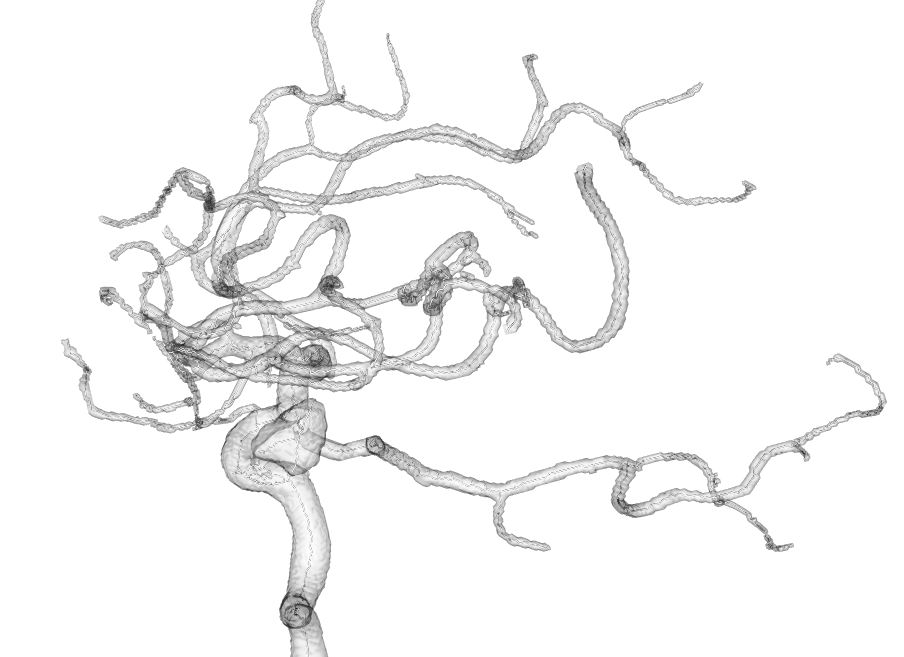
\includegraphics[scale=0.4]{fig/skeleton-transparent-segmented}
	\caption{Skeleton view with transparent segmented mesh.}
	\label{fig:skeleton-transparent-segmented}
\end{figure}


Additionally, for any skeleton view, a transparent segmented mesh can be shown by pressing "0" key. It will be hidden after pressing "0" again.

\section{Using the Spline Widget}

